% Chapter Template

\chapter{Introducción general} % Main chapter title

\label{INTROGEN} % Change X to a consecutive number; for referencing this chapter elsewhere, use \ref{ChapterX}

%----------------------------------------------------------------------------------------
%	SECTION 1
%----------------------------------------------------------------------------------------

La Ecología estudia las interacciones entre especies y entre ellas  y su entorno. Como rama de la Biología, tiene un desarrollado sentido de la clasificación y denomina a las de la primera clase \textit{bióticas} y \textit{abióticas} a las de la segunda. La gama de las bióticas es extensa, pero también se reduce a unas pocas categorías. En la \textit{depredación} una especie se beneficia y otra resulta perjudicada, como en el \textit{parasitismo}, mientras que en la \textit{competencia} los individuos, ya sean o no de la misma especie, disputan un mismo recurso. Estos tres tipos de relaciones se caracterizan por la realimentación negativa, resultan perjudiciales para una de las partes y beneficiosas para la otra. 

Si una de las especies obtiene beneficio pero para la otra es neutral se trata de \textit{comensalismo}. Finalmente, si la relación es positiva para ambas especies, es \textit{mutualismo}. En Ecología se contemplan estas relaciones desde un punto de vista de funcional y mecanicista \cite{rockwood2006introduction}, atendiendo sobre todo a los flujos de intercambio de materia, energía o servicios.

El conjunto de interacciones crea sistemas de gran complejidad. La dinámica de las poblaciones, puede describirse utilizando modelos matemáticos. Además, en las últimas dos décadas, la ciencia de redes ha contribuido al conocimiento de las comunidades ecológicas aplicando sus propias técnicas de análisis. Estas descripciones, fundamentadas en modelos y propiedades topológicas, son fenomenológicas \cite{van2010ethical}.

Los distintos enfoques metodológicos suponen a veces dificultades de comunicación, pero se enriquecen. En esta tesis se plantean contribuciones al estudio del \textit{mutualismo} desde el modelado matemático y la ciencia de redes, intentando no perder de vista su significado biológico.

\section{El mutualismo en ecología}

El término \textit{mutualismo} tuvo su origen en economía política a principios del XIX, relacionado con distintas concepciones utópicas. Fue el filósofo Pierre Joseph Proudhon el que hizo del mutualismo el eje de su teoría social y económica.

\enquote{\itshape [Mutualismo es] un sistema de equilibrio entre fuerzas libres, en el cual está cada una segura de gozar de los mismos derechos bajo la condición de llenar los mismos deberes, y 
de obtener las mismas ventajas a cambio de los mismos servicios} \cite{proudhon1868capacite}.

La idea de beneficio compartido fue trasladada al campo de la biología por el parasitólogo belga Pierre-Joseph van Beneden \cite{boucher1982ecology}, que escribió:

\enquote{\itshape Al lado [de los parásitos y comensales] hay otros que se prestan mutuamente servicios [..]. Creemos que es más justo llamarles Mutualistas} \cite{van1878commensaux}.

El mutualismo puede adoptar varias formas e intensidades. La característica que lo diferencia del resto de relaciones ecológicas es la cooperación entre especies mediante que intercambian servicios o bienes \cite{bronstein2001exploitation}.


%-----------------------------------
%	SUBSECTION 1
%-----------------------------------
\subsection{Tipos de mutualismo}
	
Las relaciones mutualistas pueden clasificarse según distintos criterios. Por el \textbf{tipo de convivencia}, se diferencia el \textit{mutualismo de simbiosis}. Las especies solo pueden vivir en una relación íntima, como las que se estableces entre numerosas especies de animales y su flora intestinal o entre bacterias y virus \cite{moran2005players}. Si, por el contrario, no hay una convivencia permanente se habla de \textit{mutualismo no simbiótico}.
	
Atendiendo a la \textbf{naturaleza del beneficio recibido}, puede ser de bienes o servicios. La polinización pertenece al primer tipo. Los animales (invertebrados en su mayoría, pero también pequeños pájaros y murciélagos) se alimentan de polen o néctar y actúan a cambio como vectores de fertilización de las plantas. La biología de la polinización es muy rica. En ocasiones, las ceras o aceites florales pueden servir para la construcción de nidos, y algunas especies de flores han desarrollado engaños para los insectos que no reciben en esa situación ningún bien a cambio \cite{rech2014biologia}.

\begin{figure}[h!]
\centering
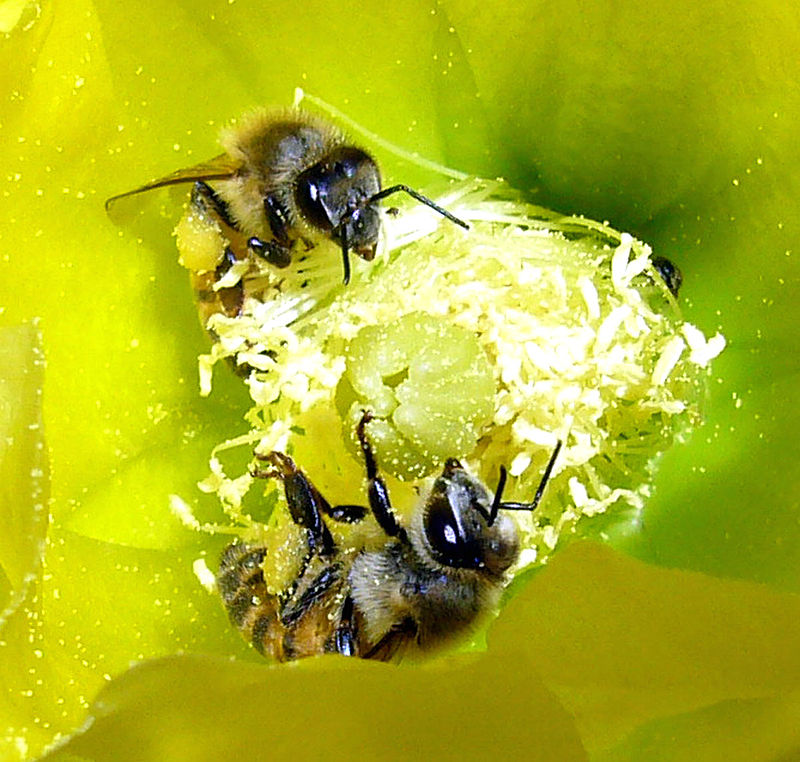
\includegraphics[scale=0.33]{Figures/INTRO_Pollination.jpg}
\caption{\textit{Apis mellifera} libando en una flor de \textit{Opuntia basilaris}, California (Estados Unidos). Fotografía de Jessie Eastland, \small{\texttt{CC BY-SA 3.0}}.}
\label{fig:VIS_bipartito_SD_001}
\end{figure}

Las comunidades de plantas y dispersores de semillas funcionan con el mismo esquema de intercambio de alimentación por servicio. Los frugívoros obtienen comida y en compensación reparten las semillas de la planta. Este tipo de mutualismo se registra sobre todo en los trópicos \cite{bascompte2007plant, estrada2012frugivores}.
	
Aunque menos comunes, también hay intercambios de recurso por recurso, como entre la bacterias del tipo \textit{Rhizobium} y las leguminosas a cuyas raíces se fijan. La bacteria proporciona nitrógeno a la planta y se alimenta de los azúcares que esta produce \cite{lindstrom2010biodiversity}.
	
Finalmente, el intercambio de servicio por servicio es la base de simbiosis como la de las anémonas con los peces y crustáceos que se han adaptado a vivir entre sus tentáculos venenoso. La anémona protege al huésped de los depredadores y a cambio este limpia sus parásitos \cite{mebs2009chemical}.

Otra distinción se basa en la \textbf{importancia vital para los actores}. En el \textit{mutualismo obligatorio} cada especie requiere del concurso de la otra para subsistir. Se suelen citar los ejemplos de yuca y sus polillas \textit(Prodixidae) o el ya citado de la anémona, aunque hay dudas de que sean absolutamente obligatorios \cite{briand1982phylogenetic, addicott1995cheating}. Está muy asociado a una gran especialización y coevolución de los mutualistas. En el \textit{mutualismo facultativo}, la relación no tiene ese carácter esencial. Es el más común en las comunidades de plantas y polinizadores \cite{geib2012tracing}.

Una última distinción se basa en la \textbf{recepción directa o indirecta del beneficio}. El \textit{mutualismo directo} es el más común, pero a veces interviene una tercera especie que
intermedia entre las dos. Boucher, James y Keeler exponen diversos ejemplos en su artículo ya citado. Desde un punto de vista de teoría de redes este \textit{mutualismo directo} es una composición de dos pares de relaciones.


\begin{figure}[h!]
\centering
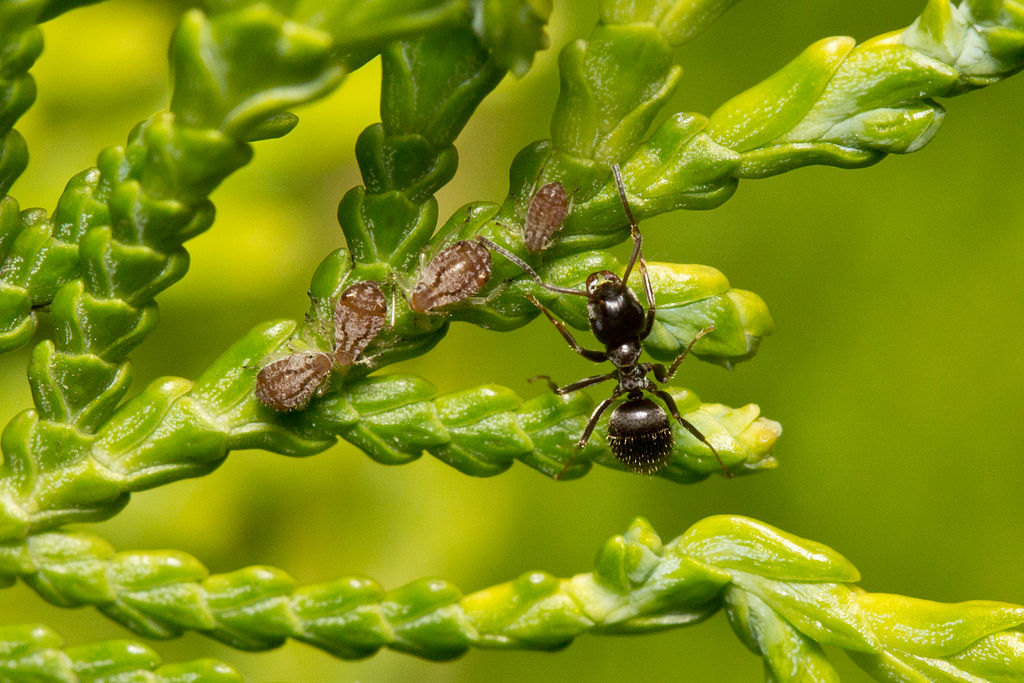
\includegraphics[scale=1]{Figures/INTRO_Lasius_niger_y_Cinara_tujafilina_en_Thuja_occidentalis.jpg}
\caption{\textit{Lasius niger} cuidando de varios ejemplares de \textit{Cinara tujafilina} sobre hojas de la conífera Tuya del Canadá \textit{Thuja occidentalis}. Fotografía de Carlos Delgado, \small{\texttt{CC BY-SA 3.0}}.}
\label{fig:VIS_bipartito_SD_001}
\end{figure}

Los insectos sociales han desarrollado formas de mutualismo muy elaboradas. En la relación entre hormigas y áfidos se intercambia un servicio (protección) por alimento (ligamaza) \cite{volkl1999ant}. Bajo determinadas circunstancias la relación se transforma en depredación de ejemplares de los primeros por las segundas, con una forma de explotación muy similar a la que se estableció en el Neolítico entre el ser humano y animales domesticados como la oveja. Otras especies cultivan hongos en sus hormigueros \cite{mueller2001origin}, en un comportamiento que también se asemeja a la relación de mutualismo que supone la agricultura.

A veces, las relaciones son complejas. Las hormigas actúan como protectoras de las acacias de las que reciben alimento y también protección contra depredadores con las púas de estos árboles \cite{raine2002spatial}. Las asociaciones entre \textit{mirmecofitas} y hormigas son muy especializadas y de naturaleza simbiótica \cite{djieto2004symbiotic}.También se documenta un tipo de mutualismo indirecto entre robles y hormigas, mediado por áfidos. La abundancia de estos no daña al árbol y beneficia a las hormigas, que a su vez, actúan como defensa frente a insectos que deterioran las bellotas \cite{ito1991indirect}.


%----------------------------------------------------------------------------------------
%	SECTION 2
%----------------------------------------------------------------------------------------

\section{Redes en ecología}

Sed ullamcorper quam eu nisl interdum at interdum enim egestas. Aliquam placerat justo sed lectus lobortis ut porta nisl porttitor. Vestibulum mi dolor, lacinia molestie gravida at, tempus vitae ligula. Donec eget quam sapien, in viverra eros. Donec pellentesque justo a massa fringilla non vestibulum metus vestibulum. Vestibulum in orci quis felis tempor lacinia. Vivamus ornare ultrices facilisis. Ut hendrerit volutpat vulputate. Morbi condimentum venenatis augue, id porta ipsum vulputate in. Curabitur luctus tempus justo. Vestibulum risus lectus, adipiscing nec condimentum quis, condimentum nec nisl. Aliquam dictum sagittis velit sed iaculis. Morbi tristique augue sit amet nulla pulvinar id facilisis ligula mollis. Nam elit libero, tincidunt ut aliquam at, molestie in quam. Aenean rhoncus vehicula hendrerit.

\subsection{Redes mutualistas}
Morbi rutrum odio eget arcu adipiscing sodales. Aenean et purus a est pulvinar pellentesque. Cras in elit neque, quis varius elit. Phasellus fringilla, nibh eu tempus venenatis, dolor elit posuere quam, quis adipiscing urna leo nec orci. Sed nec nulla auctor odio aliquet consequat. Ut nec nulla in ante ullamcorper aliquam at sed dolor. Phasellus fermentum magna in augue gravida cursus. Cras sed pretium lorem. Pellentesque eget ornare odio. Proin accumsan, massa viverra cursus pharetra, ipsum nisi lobortis velit, a malesuada dolor lorem eu neque.

Phasellus fermentum magna in augue gravida cursus. Cras sed pretium lorem. Pellentesque eget ornare odio. Proin accumsan, massa viverra cursus pharetra, ipsum nisi lobortis velit, a malesuada dolor lorem eu neque.

\subsection{Tendencias actuales en el estudio de las redes mutualistas}
Morbi rutrum odio eget arcu adipiscing sodales. Aenean et purus a est pulvinar pellentesque. Cras in elit neque, quis varius elit. Phasellus fringilla, nibh eu tempus venenatis, dolor elit posuere quam, quis adipiscing urna leo nec orci. Sed nec nulla auctor odio aliquet consequat. Ut nec nulla in ante ullamcorper aliquam at sed dolor. Phasellus fermentum magna in augue gravida cursus. Cras sed pretium lorem. Pellentesque eget ornare odio. Proin accumsan, massa viverra cursus pharetra, ipsum nisi lobortis velit, a malesuada dolor lorem eu neque.

Phasellus fermentum magna in augue gravida cursus. Cras sed pretium lorem. Pellentesque eget ornare odio. Proin accumsan, massa viverra cursus pharetra, ipsum nisi lobortis velit, a malesuada dolor lorem eu neque.

%----------------------------------------------------------------------------------------
%	ESTRUCTURA DE LA TESIS
%----------------------------------------------------------------------------------------

\section{Estructura de la tesis}
Morbi rutrum odio eget arcu adipiscing sodales. Aenean et purus a est pulvinar pellentesque. Cras in elit neque, quis varius elit. Phasellus fringilla, nibh eu tempus venenatis, dolor elit posuere quam, quis adipiscing urna leo nec orci. Sed nec nulla auctor odio aliquet consequat. Ut nec nulla in ante ullamcorper aliquam at sed dolor. Phasellus fermentum magna in augue gravida cursus. Cras sed pretium lorem. Pellentesque eget ornare odio. Proin accumsan, massa viverra cursus pharetra, ipsum nisi lobortis velit, a malesuada dolor lorem eu neque.
